\documentclass[sigconf,nonacm, 11pt]{acmart}
\usepackage[utf8]{inputenc}
\usepackage[english]{babel}
\usepackage{multirow}
\usepackage{amsmath}
\usepackage{amsfonts}
\usepackage{algorithm}
\usepackage{algorithmic}
\usepackage{tabularx}
\usepackage{mathtools}

\DeclarePairedDelimiter\floor{\lfloor}{\rfloor}

\begin{document}

\title{Semi-automatic evaluation of German party manifestos}

\author{Tobias Kalmbach}
\affiliation{%
  \institution{University of Ulm}
  \streetaddress{Helmholtzstraße 16}
  \postcode{89081}
  \city{Ulm}
  \state{Baden-Württemberg}
  \country{GER}
}
\email{tobias.kalmbach@uni-ulm.de}

\author{Fabian Karl}
\affiliation{%
  \institution{University of Ulm}
  \streetaddress{Helmholtzstraße 16}
  \postcode{89081}
  \city{Ulm}
  \state{Baden-Württemberg}
  \country{GER}
}
\email{fabian.karl@uni-ulm.de}

\author{Tim Knittel}
\affiliation{%
  \institution{University of Ulm}
  \streetaddress{Helmholtzstraße 16}
  \postcode{89081}
  \city{Ulm}
  \state{Baden-Württemberg}
  \country{GER}
}
\email{tim.knittel@uni-ulm.de}

\author{Nicolas Zellner}
\affiliation{%
  \institution{University of Ulm}
  \streetaddress{Helmholtzstraße 16}
  \postcode{89081}
  \city{Ulm}
  \state{Baden-Württemberg}
  \country{GER}
}
\email{nicolas.zellner@uni-ulm.de}

\renewcommand{\shortauthors}{T.Kalmbach, F.Karl, T.Knittel, N.Zellner}

\begin{abstract}
    % Vergleich verschiedene topic clustering methoden
    % errichten pipline für semi-automatische ausertung 
    % bieten ein tool als webinterface an
    The ability to automatically extract a set of relevant and unique topics from large text corpora has a wide range of applications. In our work, we look at the domain of political texts using the example of party programs for the German federal elections in 2021. To determine the best possible result for our specific use case, we compare a number of topic clustering approaches. 
    Based on this knowledge, we implement a pipeline for the semi-automatic evaluation of party programs and even offer a tool for this in the form of a web interface\footnote{\url{https://tadl.kalmbach.dev}}, so that information can be transferred  to the voters on the basis of this evaluation.
\end{abstract}


\keywords{NLP, LDA, HDP, BERT, Politics, Social Science, Topic Mining, Text Embedding, Text Classification}



\maketitle


% include sections

\section*{Goal of this paper}
This paper and by extension this project is by no means intended to present groundbreaking research or results. This was the first encounter with Natural Language Processing and Data Science for all of us and the first formal scientific paper for some of us.

Therefore, the goal of this paper is to a) gain a rough and general understanding of Natural Language Processing and b) extend our experience with scientific writing. 

\section{Introduction}

Politics is one of the most discussed, controversial and at the same time complex fields in society.
With so many different parties advocating their positions on a wide range of issues, it's easy to lose track of what's going on. During the election campaign, many media outlets in Germany try to summarize their positions in order to inform people about current, controversial issues through interviews, news broadcasts or inviting some politicians to discuss.

Addressing this problem and making politics more accessible and less time-consuming by simplifying the views of different parties on policy issues without loss of information is a complex goal to achieve. It is difficult to inform oneself independently since several sources must be checked for each statement in order to prevent a statement being misunderstood or even faked. The complexity of this process is increased by the fact that in many instances the candidates' statements are not taken from their official websites and are often completely different from their party's own program.   Therefore, it is necessary to take a deeper look into the election programs of the parties, since it is the only source in which the parties themselves express their position and all issues are contained in a single document. 

In order to present the opinions of different parties in a more approachable way for an interested citizen, an interactive solution is quite suitable. There are some approaches such as Wahl-O-Mat\footnote{\url{https://www.wahl-o-mat.de}}, which curate questions and let the press spokespersons of the parties answer them. However, this approach has the problem that the topics and weighting are determined by the editors of Wahl-O-Mat and do not correspond to the party-political weighting. To solve this problem, our work presents an application that identifies topics and enables users to compare the different parties based purely on the party programs. By giving the public an immediate and unbiased overview of the party positions, we hope to present information that is useful to journalists, citizens and politicians.

To achieve the best possible result, we combine different state-of-the-art approaches for topic modeling in our application. 

In the following Section, we will give a brief overview of related work. Next, we present the concepts of models that are applied in our work. Finally, we present our implementation, which is broken down into five parts: preparation, procedure, results, discussion and the presentation of our web interface. 



\section{Related Works}\label{sec:related_works}
Many applications in natural language processing are based on topic models. In addition, various approaches of topic modeling in subjects like social network, software engineering, linguistic science and more have been published. 

Whereas LDA model extracts latent topics by being integrated for measuring probabilities over a collection of documents. In NLP it facilitates approaches in different sectors like sentiment analysis or semantic knowledge inference in online news media \cite{6033626}, and much more. Pretrained BERT models enable bidirectional representations unlike recent language representation, typically left-to-right language models \cite{DevlinPres}. Its variable fine-tuning capability allows more difficult approaches like multilingual argument mining \cite{toledo2020multilingual} or detect fake news based on social bot activities like during the COVID-19 Pandemic \cite{9666618}.
The works in \citet{zirn2014multidimensional} and \citet{koh2021predicting} focus on social science with Latent-Dirichlet Allocation (LDA) models and BERT models respectively, as used in this work. 

\citet{zirn2014multidimensional} is an extension of the works from \citet{stuckenschmidt2012multi} and based on its approaches. In it, the authors present a multidimensional thematic analysis of political texts, political manifestos and transcripts as well as speeches in Germany since 1990. Focusing on the manifestos and transcripts, this work uses two different models for evaluating the political texts which are then compared on the outcome. For data preparation, the text is split automatically via TextTilling into topically coherent sub-parts. Then the cosine similarity  between adjacent token-sentences is integrated which is later also used as scheme for measuring the following step. Finally, similarity-dependent change boundaries between token sentences are identified. Based on the standard LDA more detailed in \citet{newman2009distributed,blei2003latent} and will follow in Section 3, the two different models used are Labeled LDA and Logic LDA.
While for the labeled LDA a relation between topics and labels is created via Bernoulli coin-toss in a heuristic way, the logic LDA combines word-document statistics like in standard LDA and domain knowledge
rules as in Markov Logic Networks.
The results from the two variations, a governing party which has got more similarity to the ministries topic and who gets the actual seat within parties program similarity, are compared with a baseline and a majority baseline for specifying a assignment of party closeness and given ministry position. Finally overall parties manifesto similarity in percentage is determined.
%Baseline majority is based on the acceptance that the party with the higher share has got all ministries which makes up the first evaluation in the paper, comparing overall governing parties texts similarity including seed words measuring to the ministry sector as a topic an actual given a party member the ministry position. Second is the overall parties manifesto similarity in percentage of 5 parties.
\\
The second work, \citet{koh2021predicting}, introduces different BERT models and applies those on political manifestos. Oriented on the approaches from \citet{abercrombie2019policy} the F1-score  is integrated for weighting performance of different text analysing models on political texts \cite{zhang2015estimating}. \citet{koh2021predicting} use the state-of-the-art BERT models with bidirectional gated recurrent units (GRU) models as well as deep convolutional neural network (CNN) models. They were also compared to other models like Multinomial Naive Bayes or support vector machines (SVM). The outcomes were that there is no significant wide-range difference between those techniques over low epoch rate. If it comes to increasing following generations the deep convolutional model shows best performance. Before training, data preparation is done by stemming and lemmatizing party manifestos and subsequently splitting them into quasi-sentences which are individual statements, not spanning more than one grammatical sentence.
The used principle of the BERT-CNN model here is based on the BERT BASE tokenizer, in that it uses a masked language model which allows unidirectional constraints to overcome restrictions. Filtering with convolutional filters, results in a given document setting a rectified linear activation function. Next, a 1D-max pooling layer and  a dropout layer for preventing overfitting during training is integrated. In summary, neural networks performance over policy domains yield the best approach.
%Finally, performance rates, including different policy domains and preferences, are calculated. It turns out that including a deep learning progress with a neural network is the best in overall performance regarding accuracy and loss over increasing generations or epochs of training on topics with a given data set.

\section{Models for topic mining}\label{sec:models}
As seen in the related work chapter different models can be used for topic modeling in the sector of social science. In the following, the used models are presented, namely the Latent Dirichlet Allocation (LDA) model, Hierarchical Dirichlet Process (HDP) model and the Bidirectional Encoder Representations from Transformers (BERT) model, allowing to relate several topics in a mathematical context. A concise list of variables can be found in Table \ref{tab:variable_table}.

\subsection{Latent Dirichlet Allocation Model}
Latent Dirichlet Allocation (LDA), introduced by \citet{blei2003latent}, is a generative probabilistic model for data sets, specifically text. LDA aims to extract topics from the given corpus as well as new documents inexpensively.
The central thesis is that texts are represented as random mixtures of latent subjects, each of which is defined by a word distribution. This means each topic is represented by certain words which, taken together, form a subject. The text, in turn, is modeled by several subjects, each with a certain probability that models how likely the topic relates to the text.

It's critical to distinguish between LDA and traditional clustering models.
Most clustering algorithms restrict a document to a single topic, whereas LDA utilises three layers of Bayesian modeling and samples the topic node multiple times throughout a document, allowing documents to be associated with multiple themes. 

For this reason, it is a viable option for our application.
Party programs cover a wide range of topics, and the representative terms can accurately represent the content.
In Section \ref{sec:implementation}, the implementation, evaluation, and usefulness of this model will be considered. 

\subsection{Mathematical Basis}
Following the general introduction of the LDA model, we now present the mathematical context of integrating Dirichlet distributions for topic analysis. This chapter is based on \citet{newman2009distributed} and \citet{teh2006hierarchical, teh2004sharing}. In LDA the data set is given by $D$ documents which are individually integrated in the model containing $K$ not immediately recognizable topics. In this context, the data set is a vocabulary of $W$ multinomially distributed words. Integrating a statistical approach with a Bayesian formula the result is an A-Priori-distribution called the Dirichlet distribution. We define a mixing ratio $\Theta_j$ on document $j$ and a Dirichlet distribution including the parameter $\alpha$ which satisfies the concentration.
Next, it is necessary to define a probability $\Theta_{k|j}$ for the occurrence of a word $i$ in the regarded document $j$ while extracting a topic $z_{ij}=k$. The next definition we need is the probability $\Phi_{w_{ij}}$ of a word $x_{ij}$ drawn from the topic being linked to that on value w. After that we declare the word-topic distribution $\Phi_k$ as a Dirichlet distribution with parameter $\beta$ placed on it. In summary we have declared following relations for LDA:
\begin{equation}\label{eq:lda_first}
    \Theta_j\sim\mathbf{D}[\alpha] = [\Theta_{1|j},...,\Theta_{K|j}]\sim\mathbf{D[\alpha,...,\alpha]},
\end{equation}
\begin{equation}\label{eq:lda_second}
    \Phi_k\sim\mathbf{D}[\beta] = [\Phi_{1|k},...,\Phi_{W|k}]\sim\mathbf{D}[\beta,...,\beta],
\end{equation}
\begin{equation}\label{eq:lda_third}
    z_{ij}\sim\Theta_j,\ x_{ij}\sim\Phi_{z_{ij}}
\end{equation}

With \eqref{eq:lda_first}, \eqref{eq:lda_second} and \eqref{eq:lda_third} it is possible to count words belonging to a topic in one document $j$:
\begin{equation}\label{eq:lda_fourth}
    N_{kj}=\sum_{w=x_{ij}}N_{wkj},
\end{equation}
\begin{equation}\label{eq:lda_fifth}
    N_{wk}=\sum_{j}N_{wkj}
\end{equation}
The overall Dirichlet distribution with \eqref{eq:lda_fourth} and \eqref{eq:lda_fifth} is:
\footnotesize
\begin{equation}
     \begin{split}
     &p(x,z,\Theta,\Phi|\alpha,\beta)
     \sim\\
     &\prod_{j}\frac{\Gamma(K\alpha)}{\Gamma(\alpha)^K}\prod_k\Theta_{k|j}^{N_{kj+\alpha-1}}\prod_k\frac{\Gamma(W\beta)}{\Gamma(\beta)^W}\prod_w\Phi_{w|k}^{N_{wkb}+\beta-1}
     \end{split}
\end{equation}
\normalsize
% As basic assumptions for both(Variational methods & MCMC)
Having defined the Dirichlet distribution, there are two different ways for calculating posterior distribution and approximating Bayesian inference for a given word $x$. It is possibile to use variational methods like as Markov Chain Monte Carlo (MCMC) algorithms. 

$x$ is the given word and $z$ the latent topic assignment with mixing proportion $\Theta$ and topics $\Phi$ as before.
% In cite 4 (Blei) variational methods
The variational method approach from \citet{blei2003latent} first calculates the posterior distribution of hidden variables with
\begin{align}
    \begin{split}
    &p(x|\alpha,\beta)=\\
    &\frac{\Gamma(\sum_i\alpha_i)}{\prod_i\Gamma(\alpha_i)}\int_K(\prod_{i=1}^{k}\Theta_i^{\alpha_i-1})(\prod_{n=1}^N\sum_{i=1}^k\prod_{j=1}^J(\Theta_i\beta_{ij}^{x_{ij}})) d\Theta
    \end{split}
\end{align}
After this the convexity-based variational inference with Jensen's inequality omits fitting lower bounds for the logarithmic probabilities. Overall, an optimisation approach is followed during approximation with a variational parameter indexing lower bounds for yielding the tightest solution. Like in the graphical model we assume this model as tree with edges and nodes. The edges between $\Theta$, $z$ and $x$ are dropped in the next step to get a new family of distributions on the latent variables as our first variational distribution:
\begin{align}
    q(\Theta,z|\gamma,\Phi)=q(\Theta|\gamma)\prod_{n=1}^Nq(z_n|\Phi_n),
\end{align}
where $\gamma$ is placed on $\Theta$ and ($\Phi_1$,...,$\Phi_N$) is known as the multinomial parameters representing the free variational parameters. 
The optimization progress follows with Kullback-Leibler divergence between Eq. (7) and (8). The optimization problem:
\begin{align}
    \begin{split}
    &(\gamma^{*},\Phi^{*})=\\
    &arg\{min_{(\gamma,\Phi)}\{D(q(\Theta,z|\gamma,\Phi)||p(\Theta,z|x,\alpha,\beta)) \}\}
    \end{split}
\end{align}
is minimized during an iterative process for getting the derivatives. These are then set equal to zero to obtain a pair of updated equations:
\begin{align}
    \Phi_{ni}\sim\beta_{ix_n}exp\{E_q[log(\Theta_i)|\gama]\} \\
    \gamma_i=\alpha_i+\sum_{n=1}^N\Phi_{ni}
\end{align}
and compute as well the expectation within the multinomial update: 
\begin{align}
    E_q[log(\Theta_i)|\gamma]=\Psi(\gamma_i-\Psi(\sum_{j=1}^k\gamma_j)).
\end{align}
$\Psi$ can be seen as the first derivative of the logarithmic-gamma function. For a more detailed look of the calculation of the equations (9), (10), (11) and (12) have a look in the appendix in \citet{blei2003latent}. Based on the formulas above the approximation to the posterior distribution can be realized for a given data-set.
\\\\
%In tomotopy MCMC
Approximating inference with MCMC given $\Phi$ and $\Theta$ are integrated in (6) which is called collapsing. During this process the latent topics z are sampled and the current state of one variable $z_{ij}$ is omitted with following conditional probability:
\begin{align}
    p(z_{ij}=k|z^{\neg{ij}},x,\alpha,\beta)\sim\frac{N_{wk}^{\neg{ij}}+\beta}{\sum_wN_{wk}^{\neg{ij}}+W\beta}(N_{kj}^{\neg{ij}}+\alpha)
\end{align}
In general observed topics conditional probability is computed by excluding the assigned word in place \textit{$x_{ij}$} with $\neg{ij}$.
\\\\

\begin{figure}[h]
    \centering
    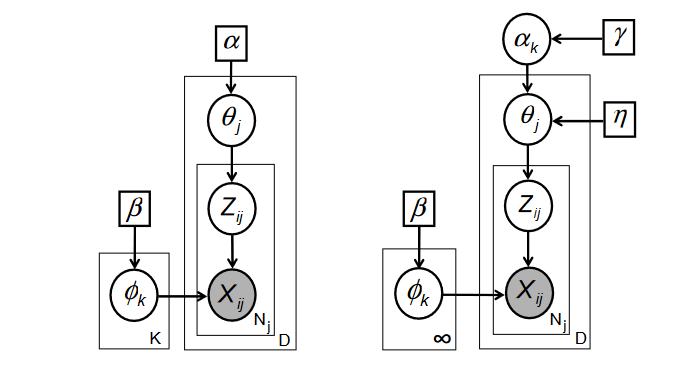
\includegraphics [width=\linewidth]{resources/LDAAndHDP.png}
    \caption{Graphical models for LDA (left) and HDP (right) \citet{newman2009distributed}}
    \label{fig:lda_hdp}
\end{figure}

\subsection{Hierarchical Dirichlet Process Model}
With the works in \citet{newman2009distributed} and \citet{teh2006hierarchical,teh2004sharing} the basic concept of HDP follows. To understand the hierarchical concept it is necessary to have an overview of basic Dirichlet Processes (DP). We define a measurable space $(\Theta, B)$ and a $\alpha_0 \in \matthbb{R}^+$. Let $G_0$ be a probability measure on $(\Theta, B)$. A arbitrary partition ($A_0,..,A_n$) of $\Theta$ with n $\in \matthbb{N}$ and n$<\infty$ the random vector included in a random probability measure G over $(\Theta, B)$ distributed with concentration parameter $\alpha_0$ is called the \textit{Dirichlet process} $DP(\alpha_0,G_0)$.
\begin{align}
    (G(A_1),...,G(A_n)) \sim Dir(\alpha_0G_0(A_1),...,\alpha_0G_0(A_n))
\end{align}
On this basis the approach of the hierarchical model combines multiple DP where a global random probability measure $G$ predetermines the basic concept of the following probability measures hierarchically structured.

Figure \ref{fig:lda_hdp} serves as a visualisation of the mathematical basis mentioned before. On this guidance the \textit{tomotopy} framework integrates both models similarly.
With right model in Figure \ref{fig:lda_hdp}, HDP, it is possible to progress by sharing clusters among related groups on multiple text documents in general.

%With the right model in Figure \ref{fig:lda_hdp}, \citet{newman2009distributed} and \citet{teh2004sharing} we clear the integration of this concept within progress other sharing cluster among related groups on multiple text documents in a general way realized in \textit{tomotopy} framework.

The general process in HDP is similar to the LDA model with simple changes. Our data set is $D$ documents with $K$ latent topics.
Here $\alpha_K$ is the $alpha$ of the global process in the highest level of the hierarchy. The Dirichlet with parameter $\alpha_{K}$ is applied on concentration $\eta$ which samples it with parameter $\frac{\eta}{K}$. Following, we omit topic mixture with parameter $\eta\alpha_K$ and word distribution like before:
\begin{align}
    \begin{split}
    &\alpha_K\sim\mathbf{D}[\gamma/K],\ \Theta_j\sim\mathbf{D}[\alpha],\ \Phi_k\sim\mathbf{D}[\beta],\\ &z_{ij}\sim\Theta_j,\ x_{ij}\sim\Phi_{z_{ij}}
    \end{split}
\end{align}
Subsequently, the direct assignment sampler for HDP is omitted for getting the posterior distribution calculated in \citet{teh2006hierarchical}. Resulting, like in LDA $\Theta$ and $\Phi$ are integrated in (6). Finally with those approaches we end up in  conditional distribution for latent topic assignments:
\begin{align}
    \begin{split}
    &p(z_{ij}=k|z^{\neg{ij}},x,\alpha,\beta,\eta)\sim\\
    &\begin{cases}\frac{N_{wk}^{\neg{ij}}+\beta}{\sum_{w}N_{wk}^{\neg{ij}}+W\beta}(N_{kj}^{\neg{ij}}+\eta\alpha_k),\ $k= prev. k$\\
    \frac{\eta\alpha_{new}}{w}, $ k=k_{new}.$\\
    \end{cases}
    \end{split}
\end{align}

\begin{table}[h]
    \begin{tabular}{|p{1cm}||p{6.5cm}| }
        \hline
        variable & description\\
        \hline
        D & number of documents\\
        W & number of different words in vocabulary\\ 
        N & number of words in data-sets\\
        K & number of topics\\
        $x_{ij}$ & $i^{th}$ investigated word in document j\\
        $z_{ij}$ & topic allocated to $w_{ij}$\\
        $N_{wk}$ & Counter: word allocated to topic\\
        $N_{kj}$ & Counter: topic allocated in document\\
        $\Phi_k$ & probability of word being suitable for topic t\\
        $\Theta_j$ & probability of topic being suitable for document j\\
        $\alpha$ & probability measure parameter placed on $\Theta_j$ \\ 
        $\beta$ & probability measure parameter placed on $\Phi_k$ \\
        $\gamma$ & concentration parameter\\
        $\eta$ & probability measure parameter applied to $\alpha_k$ placed on $\Theta_j$\\
        \hline
    \end{tabular}
    \caption{Description of used variables \citet{newman2009distributed}}
    \label{tab:variable_table}
\end{table}
% Advantage: number of topics determined by data


% tomotopy: can use adv. of multicore CPUs (with SIMD instr. set) -> faster iter. 
% Variational Bayes(VB) used in genisms LdaModel


\subsection{BERT model}
Another approach to extracting topics from party programs was using Bidirectional Encoder Representations from Transformers (BERT). 
\subsubsection{Training}
The technology of including contextual information from both, left and right side instead of only one side guarantees better results and was first introduced with the BERT model in \citet{Devlin2019BERTPO}. This behavior allows a deeper understanding of the language model.

The goal of BERT and other BERT style model's training processes is to correctly predict missing words in sentences by their context. The BERT model therefore uses two different approaches:
\begin{enumerate}
    \item Masked LM (MLM) \\
    In this approach, 15\% of the tokens are selected and these selected tokens are replaced by the following tokens as a copy of the original token sequence:
    \begin{itemize}
        \item 80\% of the tokens are replaced by [MASK] tokens
        \item 10\% of the tokens are replaced by random words
        \item 10\% of the tokens are kept the same
    \end{itemize}
    This detailed information was first published in \citet{DevlinPres}.
    The original token and modified token sequence are then embedded into vectors which are then processed by BERTs transformer encoder layers. \hyperref[sec:transformer]{Section 3.4.2} gives a more detailed view on BERT's transformer architecture. The output vectors of the classification layer are now being multiplied with the embedding matrix, allowing the model to calculate the probabilities of each word using the softmax function 
    \begin{align}
        \sigma(\textbf{z})_i = \frac{e^{z_i}}{\sum^K_{j=1} e^{z_j}}
    \end{align}
    where \textbf{z} is the input vector of \emph{K} elements and $i \in [1,K]$.
    \begin{figure}[h]
        \centering 
        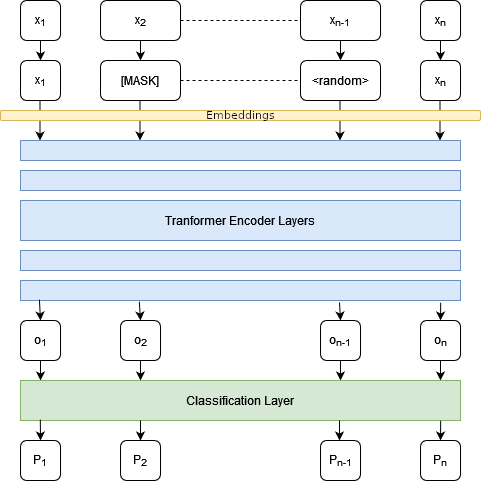
\includegraphics [width=\linewidth]{resources/BERT_MLM.png}
        \label{fig:my_label}
    \end{figure}
   
    \item Next Sentence Prediction (short NSP) \\
    Next Sentence Prediction is the process of determining whether a given sentence is the subsequent sentence to another given sentence. As an input it receives a list of pairs of two sentences of which 50\% are a combination of two subsequent sequences and the other 50\% got a random sentence as their second element without the model knowing which are which of course. The goal of the NSP model is then to identify which sentences are subsequent and which are in no positional relation. \\
    Before the input reaches the transformer model it gets preprocessed in the following steps:
    \begin{enumerate}
        \item The input is tokenized on a word basis (ex. "playing" --> ["play", "##ing"])
        \item A [CLS] token is inserted before the first sentence and a [SEP] token is inserted after each sentence.
        \item A sentence embedding layer which indicates to which sentence a token belongs.
        \item A positional embedding layer which indicates to what position a token a token belongs in the input string. This is used to represent positional relations between the input tokens.
    \end{enumerate}\\
    The sentences \emph{"my dog is cute. he likes playing"} would lead to the following output after the preprocessing steps: 
    \begin{figure}[h]
        \centering 
        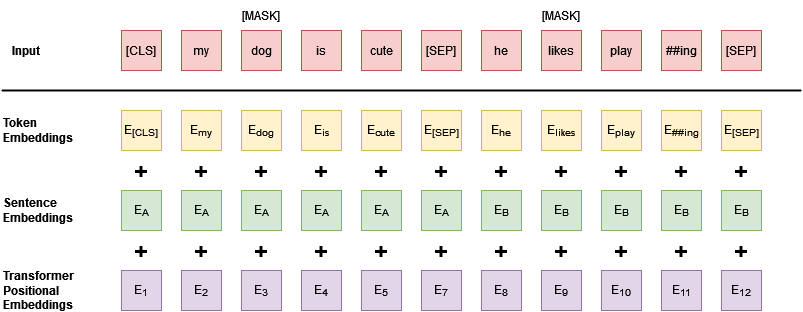
\includegraphics [width=\linewidth]{resources/NextSentence.png} \\
        \caption{\citet{Devlin2019BERTPO}. A larger version can be found in the appendix, Figure \ref{fig:next_sentence_large}.}
        \label{fig:my_label}
    \end{figure}
    \\
    The preprocessed input is then passed to the transformer model where the output is then used to calculate the probability of IsNextSequence with the softmax function.
\end{enumerate}
\subsubsection{Transformer Architecture}
\label{sec:transformer}
Transformers are the first transduction models relying entirely on self-attention mechanisms \cite{1706.03762}.
The complete architecture of one transformer is shown in Figure \ref{fig:transformer}.
\begin{figure}[h]
    \centering 
    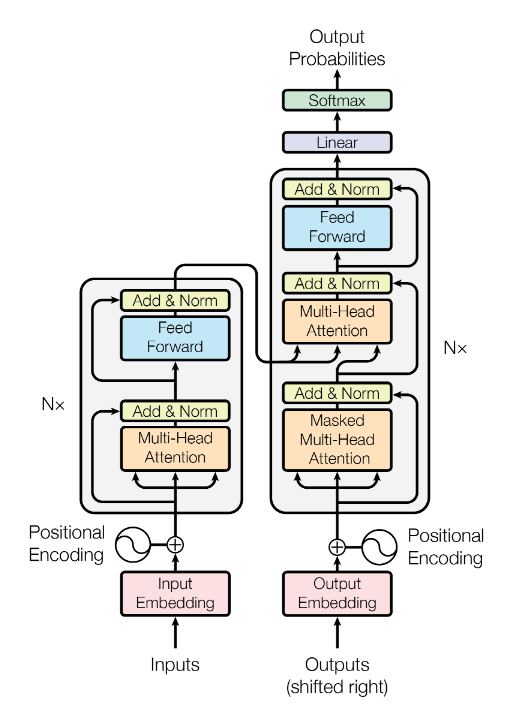
\includegraphics [width=\linewidth]{resources/Transformer} \\
    \caption{\citet{1706.03762}}
    \label{fig:transformer}
\end{figure} \\
The individual components are now being described in more detail:
\begin{itemize}
    \item \textbf{Encoder}: The encoder is shown in the left part of the figure and consists of 6 similar layers that all contain a self-attention mechanism layer and a feed-forward network layer. Every single sub-layer produces an output of dimension $d_{output} = 512$
    \item \textbf{Decoder}: The decoder (shown on the right) is pretty much similar to the encoder except for the additional maskes multi-head attention layer.
    \item \textbf{Multi-Head Attention}: The goal of an attention mechanism is to generate a weighted sum of values, where the input is a query vector and two other vectors representing key-value pairs. The multi-head attention layers are more or less the most important part of the tranformer's architecture. Their core consists of a scaled dot-product attention mechanism, which takes in three different vectors of size $d_k, d_k, d_v$, where the vector of queries and keys are of size $d_k$ and die vector of values is of size $d_v$. Since in reality the attention mechanism is applied to a set of input vectors simultaneously, the vectors are grouped in matrices. The result of the scaled dot-product attention function can then be expressed as follows: \\
    $Attention(Q, K, V) = softmax(\frac{QK^T}{\sqrt{d_k}})*V$
    \item \textbf{Feed-Forward Network}: The FFNs are basically a ReLU activation $ReLU(x) = max(0, nx)$ of a linear transition multiplied by another linear transition: \\
    $FFN(x) = max(0, xW_1+b_1)*W_2+b_2$
\end{itemize}

\section{Implementation}\label{sec:implementation}
Following the theoretical description of the used models, now we present our practical approach. This section is split into the data preparation, explaining our procedure and explicit implementations and lastly, the evaluation of our findings.

\subsection{Data Preparation}
To extract topics or corresponding arguments, we first need data. In this case we use a data-set from \href{https://kaggle.com}{Kaggle} that provides us with the manifestos of all the big parties (CDU, Grüne, SPD, FDP, AfD and Linke) competing in the 2021 German federal election. The data-set is available \href{https://www.kaggle.com/sibelius5/party-platforms-for-the-german-federal-election-21}{on Kaggle}\footnote{\url{https://www.kaggle.com/sibelius5/party-platforms-for-the-german-federal-election-21}}.


The first step in preparing our data was preprocessing. We selected to approach this task in two different ways to see which approach works better. For all our general language processing, we used \href{https://spacy.io/}{spaCy}\footnote{\url{https://spacy.io/}} with the pre-trained \texttt{de\_core\_news\_md} model provided by spaCy \footnote{\url{https://spacy.io/models/de\#de_core_news_md}}.

Firstly, we chose to use a rather explicit approach, tokenizing and lemmatizing our party manifestos with spaCy and then manually selecting what words or word types to filter out. We filtered out stop words, as is common practice, however, also all numbers, URLs, emails, currencies, party names and tokens with certain part-of-speech (POS) tags (verbs in third person singular, adpositions, pronouns and auxiliary words). After filtering all of this, we gathered simple statistics on our words, like what words were used most frequently. This was done to gain a better overview and just get started with text analytics tools in general.

As an example, Figure \ref{fig:spd_stats} shows the word frequencies for the SPD.
 
\begin{figure}[h]
    \centering
    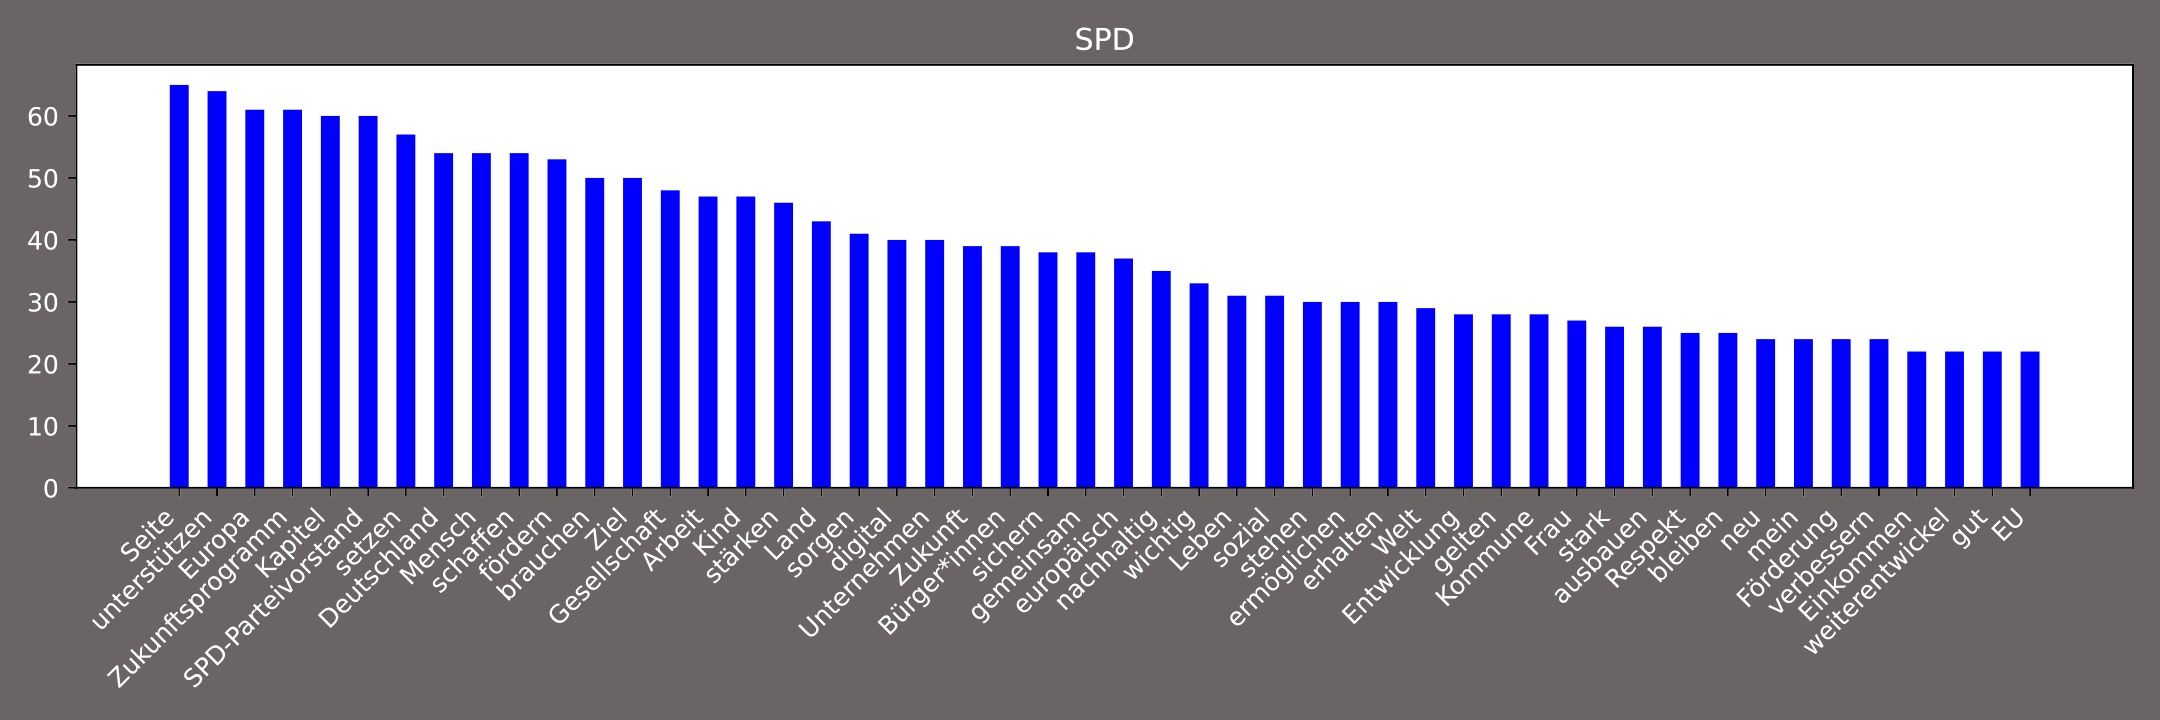
\includegraphics[width=\linewidth]{resources/graph_SPD.png}
    \caption{Word frequencies for the 50 most used words by the SPD in their 2021 federal election manifesto. A larger version can be found in the appendix, Figure \ref{fig:spd_stats_large}.}
    \label{fig:spd_stats}
\end{figure}

In our second approach, we used the \textit{simple\_preprocess} method from gensim which automatically preprocesses data. \textit{simple\_preprocess} lowercases all words and tokenizes the data. Subsequently, we removed stopwords in an extra step, using stopwords from spaCy and nltk. Both spaCy and nltk were used, as some stop words in the spacy corpus were not included in the nltk corpus and vice versa. In total the combined stopword list from spacy and nltk was comprised of 567 words. This extensive list of general stop words was extended manually, to a total size of 696 words. This addition was necessary to not affect our data negatively, as some phrases or words are used in political text and especially manifestos often, but do not usually count as stopwords (e.g. \glqq deutsch\grqq{} as in German or the respective party names). The need for additional stopwords can also be observed in Figure \ref{fig:spd_stats}, where \glqq Seite\grqq{} as in page is the most common word. Another specific word that needed to be amended was the gendered form of words with \glqq\texttt{*innen}\grqq{}, for example \glqq\texttt{Bürger*innen}\grqq{} would be transformed into \glqq\texttt{Bürger}\grqq{}. This change was necessary, as the model would remove the separating star-symbol but treat \glqq\texttt{innen}\grqq{} as a separat word. As a result, \glqq\texttt{innen}\grqq{} would often be among the most frequent word in manifestos that used this style. The left over words were then used to create bi- and trigrams for later use. In addition, the words were lemmatized and all words with POS-tags that were not nouns, verbs, adjectives and adverbs were filtered out. This procedure showed more promising results, so this now heavily processed manifesto text was used in the following steps for topic modelling.

Finally, we manually edited the formatting of party manifestos, as some manifestos did not have clear breaks between paragraphs or graphic formatting dividing a single paragraph in two separate parts. Additionally, all headlines were removed as these would be treated as parts of sentences, due to missing punctuation.

\subsection{Procedure}
In this section, we discuss our different approaches we used in our application. First, we discuss our models used for topic modelling, then how we summarized our texts and finally, our web interface.
\subsubsection{LDA for topic modeling}
We used the \href{https://radimrehurek.com/gensim/index.html}{gensim} framework \cite{rehurek_lrec} for our LDA model. Gensim works by statistically extracting patterns in the given text and linking similarities between documents thus generalizing common topics. % work out gensim better

As we only have one manifesto per Party, we split the manifesto in paragraphs and treat the paragraphs as single documents. We did this, with the premise that every paragraph in a manifesto only focuses on one general topic and thus a good estimation of the topic can be extracted for each paragraph.
For the actual LDA model we used the pre-trained model provided by gensim. The model is given a integer id representation of a each word (id2word) and with these ids a bag-of-words is created and used as our corpus. The LDA model then runs for a specified number of iterations, extracting a number of topics. We settled on 10 topics as this is recommended in literature \cite{gan2021selection} and all manifestos should at least cover 10 separate topics. Through trial and error and analyzing our results we later found five to seven topics to be optimal. We use the (\textit{pyLDAvis}) library which visualizes our topics, showing simple relations between topics and which words are grouped in one topic. As measurements for how accurate and well the model performed, we measured the perplexity and coherence. The specific results and more detailed description will follow in Section \ref{sec:lda_results}. 

As we wanted to have other data to compare our results to, we ran the same process with other models. The models we settled on were LSI and HDP. Similar to the LDA model we measured the coherence of the results. The comparison of LDA, LSI and HDP will also follow in Section \ref{sec:lda_results}. 

% gensim besser herausarbeiten
% LSI und HDP besser beschreiben


\subsubsection{HDP}
At a later point, we tested an other implementation of the HDP model by using the \textit{tomotopy} \cite{bab2min_2021_4999089} framework. This framework is based on the principles of \citet{teh2004sharing} and \citet{newman2009distributed}. With inferred topic and word distributions, the Collapsed Gibbs Sampling (CGS) supports the \textit{tomotopy} framework. Dependening on the number of documents, CGS improves the computation time. When a new topic is considered, every word in a random order will be determined and processed to open up new topics dependent on the probability of an assignment to the current topic. For more details about CGS processes and its optimization possibility look in \citet{subeno2018optimisation}. On this basis, tomotopy can make use of multicore CPUs including a SIMD (Single Instruction, Multiple Data) instruction set for faster iterations \citet{bab2min_2021_4999089}. Here the aim was creating a model to filter party manifesto and receive topics by the uncertainty in their number which is a property of the HDP model. One party manifesto was load as an \textit{Iterable String} for integrating the pretrained model of the HDP by setting it on the number of cores of the system with parameter 0. After that the \textit{burn\_in} iterations for optimization were called with a value of 500.
%Outcomes docs=1(FDP), Vocab=758,TotalWords=8385
Then the word log likelihood was set over a word range of 5000 with a step of 50 and trained with 50 iterations of Gibbs-sampling.
% HDP captures the uncertainty in the number of topics
Whole training process oriented on the model previously mentioned in Section 4 with a minimum collection frequency of documents of 5 and of words of 0. Here the initial parameter of FDPs party manifesto were the number of topics is k=10, the concentration coefficient of DP for document-table $\alpha$=0.1, the hyper-parameter of Dirichlet distribution for topic-word $\eta$=0.01 and the concentration parameter of DP for table-topic $\gamma$=1.0. The first instantiated random seed word value was 99999. After training process the concentration coefficients changed to $\alpha$=6.6722, $\gamma$=66.12 and the Dirichlet Prior on the per-topic word distribution stayed at an value of $\eta$=0.01. Overall generated outcome were 46 topics as well as tables.

\subsubsection{Topic classification on BERT embedding}
% Motivation: Wir haben keine ausgewertet daten -> unsupervised (evtl weak supervised)
% preprocessing -> aufteilen in sections (Annahme: eine sektion nur ein primäres thema)
% sections durch BERT in embedings vektoren um kontext zu schaffen
% CLuster aus LDA -> Themen mit passenden tokens
% ebenfalss in BERT
% Cosine-simularity berechenen und entsprechend zuordnen  as stated by https://dl.acm.org/doi/abs/10.1145/3366423.3380278
Since there is unfortunately no possibility to classify the topics on the basis of completely evaluated data sets for our topic, we have to work only on the basis of the party programs. The idea which we pursue for this, must first of all divide the text into meaningful parts, whereby we make the reasonable assumption that a paragraph in the text primarily revolves around a certain topic.

Based on the work of \citet{Meng2020}, our approach is the classification based on representative tokens for the respective topics. These representative tokens were chosen based on the results of our work with LDA, which yielded the best results for our data. 
We use a pre-trained BERT tokenizer and model to determine the embedding for both the representative tokens and the paragraphs to determine the proximity between the paragraphs and the topics. This model by the \citet{bert-base-german-cased}  is a German BERT implementation that was trained on 2,350,234,427 tokens gathered from a variety of data sets, including a recent Wikipedia dump and News Crawl.

A novelty of our approach is that here, we use word embedding and not only the bag-of-words model. We do not model the individual text with tokens, but instead use this concept of embedding to capture the semantics and structure of our text documents. This significantly improves the topic model and allows it to predict the topics of sections much better than just using a simple bag-of-words model.

We calculate the pairwise Cosine-Similarity in the word vector space based on these vectors to determine the topic that best reflects the paragraph. Each paragraph must be assigned a topic in this manner. For convenience reasons, we use integers as topic ids and just select the closest topic that is most relevant for our paragraph.

\subsubsection{Summary of topics}\label{sec:summary}
As our goal is to show the user a concise overview of topics discussed in the party manifestos, the simple connection of topics to sections is not sufficient. So, for each topic used in our classification, we concatenate every corresponding section gaining a combined text containing all paragraphs classified with a specific topic. This, however, still does not simplify the manifestos and at best orders the sequence of topics. Our next step was then to individually summarize all texts we created in the previous step.
An important requirement for the summary we set ourselves was the need for an extractive summary, meaning sentences in the summary can only be taken verbatim from the original text. We committed ourselves to this obligation, as we did not want to alter the statements given by the party in any way, shape or form, to guarantee reproducible and traceable results.

However, it proved very difficult to find a good model or library to summarize German texts in an extractive manner. Among others, we tested summarizing texts with a few models on huggingface, both German and English models, but did not achieve satisfying results.
After some searching we found \textit{sumy} \footnote{\url{https://github.com/miso-belica/sumy}}, a lightweight library for summarizing texts in various languages, including German. When testing \textit{sumy} with sample texts it worked a lot better than any previous attempts, so in the end we settled on \textit{sumy}. \textit{sumy} incorporates a built-in parser for plain text, files as well as HTML pages. Besides parsers \textit{sumy} offers several types of summarization methods, which can be found on GitHub \footnote{\url{https://github.com/miso-belica/sumy/blob/main/docs/summarizators.md}}. We use LSA (Latent Semantic Analysis) as it is "the most advanced method" and generally yields good results.

\subsection{Results}
In this section we present the results of our previously discussed models. First, the LDA topic modeling results and second the topic classification with BERT embeddings.
\subsubsection{LDA for topic modeling}\label{sec:lda_results}
% fdp pyldavis
% LDA, LSI, HDP vergleich 
% Grafiken einbinden
% resulate aus grafiken \cite{mimno2011optimizing}

The topic clustering with LDA was the first result we obtained during our project.
As can be seen in Figure ~\ref{fig:lda_cluster} with the example of the FDP, it is possible to use LDA to create clusters that represent the topics of the text. 
However, in our data set, the issue is that the overview of the terms contained in the cluster gives a person a natural understanding of the topic, but there is no clear representative that truly describes the cluster's topic.

\begin{figure}[h]
    \centering
    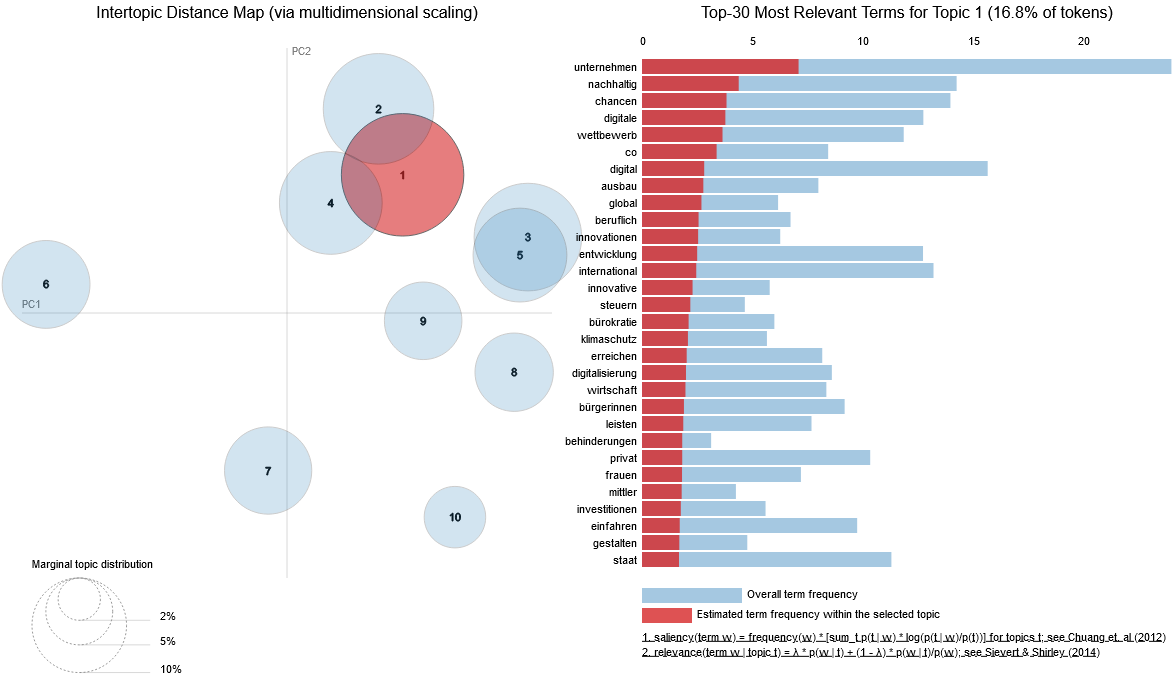
\includegraphics [width=\linewidth]{resources/fdp_cluster.png}
    \caption{LDA visualization at the example of the FDP. A larger version can be found in the appendix, Figure \ref{fig:lda_cluster_large}.}
    \label{fig:lda_cluster}
\end{figure}

Furthermore, it is evident that some topics overlap in a minor or even major way. It can also be seen that the number of topics has a strong influence on the overlap when the number of topics is adjusted, which is why we try to find the best number based on this direct consequence. The coherence score is used to accomplish this. The coherence score indicates how easily the topics can be understood by humans. In our case, the coherence score of a topic may be summarized as follows: If a topic has a high average pairwise similarity with its top $k$ word, it indicates that the topic is very coherent, and can be easily understood by humans. \cite{mimno2011optimizing}
As can be seen in Figure ~\ref{fig:coherence_score}, the coherence score for the first few topics falls\footnote{In gensim u\_mass is always negative and lower values are desirable.} disproportionately, while it continues to fall later, but due to overlaps it is no longer as meaningful. Based on this knowledge, we determine 5 to 7 topics as a good number for party programs. 

In addition, we did the same procedure with LSI and HDP but these methods do not bring us any new insights. However, since they behave the same way as LDA, this check confirms our assumption regarding the number of topics. 


\begin{figure}[h]
    \centering
    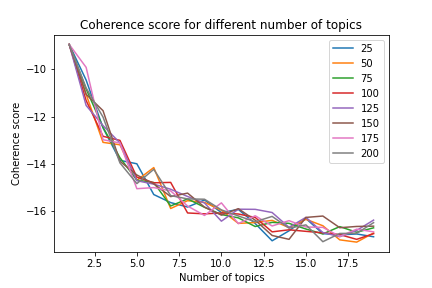
\includegraphics [width=\linewidth]{resources/coherence_score_u_mass_for_CDU.png}
    \caption{U\_MASS coherence score for the CDU. The legend shows the number of epochs for the LDA-Modell}
    \label{fig:coherence_score}
\end{figure}


\subsubsection{Topic classification on BERT embedding}
The output of our BERT implementation is a dictionary with the different parties as the keys and tuples of the most significant sentence-topic pairs as the values. This representation allows a viewer to directly obtain what a party's view on a specific political topic is.

Since the complexity of the self-attention layer inside the transformers is $O(n^2)$ the embedding-conversion is taking quite a while for all the %$\floor{\frac{|T|}{256}}$ 
chunks.

%\subsubsection{Using BERT to get the according text passages}
\subsection{Discussion}
% custom stopwords
In the context of political texts, we have encountered the problem of having a large number of words without meaning, so we decided to introduce context-dependent stopwords.
To bring the texts into a consistent presentation, these contextual stop words include the removal of all gendered language as well as phrases like "we demand..." (wir fordern). No information is lost because these words do not add any expressiveness to the passage's theme. However, we observed that removing them results in much better LDA clusters, with the strongly represented terms now being more representative of the clusters.
In selecting these stopwords, we had to be careful to remove as many as possible in order to get a good result, but also not to be too specific to these texts, so that a generalization still exists and the method could be applied to other party manifestos.

% is topic number realistic
Another finding from our research is an optimal number of 5-7 topics within a text. This finding also makes sense, since within an election the parties have to decide on a reasonable number of issues they want to address. In general, there is a trade off between having fewer, larger topics that are more general and having many, more specific topics.

% results of lda, lsi and hdp
Unfortunately, the LDA, LSI, and HDP clusters we obtain are not as valuable as we had planned for further processing of the party programs. Since it is difficult to select the right appropriate text passages from these clusters, but they assist us in the sense that we can manually evaluate them before applying the knowledge to topic classification on BERT embedding.

% classification
On this foundation, we built a classifier that produced decent results despite the lack of labeled data. There are still some obvious mismatches, but we couldn't get a better outcome by tweaking the parameters. Furthermore, those mismatches are less noticeable after the summerization.


\subsection{Web Interface}
We created a web interface to offer an easy way to interact with our results.
The web interface is a simple \href{https://vuejs.org/}{Vue} \footnote{\url{https://vuejs.org/}} application using \href{https://www.naiveui.com/en-US/os-theme}{Naive UI} \footnote{\url{https://www.naiveui.com/en-US/os-theme}} as a UI framework. The page is available at \href{https://tadl.kalmbach.dev/}{https://tadl.kalmbach.dev/}.

Using the results we gained in the previous sections, we landed on 6 topics, namely environment (Umwelt), economics (Wirtschaft), education (Bildung), society (Gesellschaft), domestic politics (Innenpolitik) and labor and social affairs (Arbeit und Soziales). Then, summaries for every topic were created as described in Section \ref{sec:summary}.

The summaries are presented with no party affiliation to offer a unbiased review. 
Even though, the summaries do not have a clear assignment, summaries can contain phrases which include the party name (e.g. "<Party> promises to ..."). As this is done in several variations and we did not want to introduce bias, we did not remove or hide this type of party affiliation, causing the statements not be entirely anonymous.

Each summary can be rated from one to five stars and after all summaries were rated, a ranking of all parties by stars their respective statements were given is presented.
After completing this for every topic, one can choose to redo the ranking, with the added option of showing directly which summary came from what party. This provides the opportunity to look into specific party manifestos if the summaries were appealing.

\section{Conclusions and future work}
In this work, we implement a pipeline to classify distinct topics based on semi-automatic evaluation of the party manifestos. To do so, we use LDA, LSI, and HDP, with LDA being particularly effective in our domain. For the final classification we use BERT embeddings. The results are not always perfect, but given that no data set with evaluated topics was used, they are quite reasonable.
In the future, it will be possible to extend this pipeline to a fully automatic evaluation by using labeled data. In addition, the topics can also be differentiated into high granular topics and possibly also into a hierarchical representation. 
Besides that, for a neutral perspective on the topics, an extension that fully anonymizes the results would be beneficial for our interface, as the texts should not reveal the party from which they originally come.
Furthermore, our web interface can be extended with other useful processing methods such as a question-and-answer function in the form of a chat.  
This should allow a flexible and user-friendly way to interact with party manifestos.


\bibliographystyle{ACM-Reference-Format}
\bibliography{references}

\appendix

\section{Distribution of work}
Generally, we tried to work in groups, so the following is an approximation, of which authors are mainly responsible for the corresponding sections. The distribution of our programming work can be found in the README of our GitLab project.

\begin{tabularx}{\linewidth}{X|X}
\textbf{Part}                                  & \textbf{Responsible author(s)} \\ \hline
Abstract                                       & Fabian Karl                    \\
1 Introduction                                 & Fabian Karl \& Tim Knittel     \\
2 Related Works                                & Nicolas Zellner                \\
3.1 Latent Dirichlet Allocation Model          & Tobias Kalmbach \& Fabian Karl \\
3.2 Mathematical Basis                         & Nicolas Zellner                \\
3.3 Hierarchical Dirichlet Process Model       & Nicolas Zellner                \\
3.4 BERT model                                 & Tim Knittel                    \\
4.1 Data Preparation                           & Tobias Kalmbach                \\
4.2.1 LDA for topic modeling                   & Tobias Kalmbach                \\
4.2.2  HDP                                     & Nicolas Zellner \& Tim Knittel \\
4.2.3 Topic classification on BERT embedding   & Fabian Karl                    \\
4.2.4  Summary of topics                       & Tobias Kalmbach                \\
4.3.1  LDA for topic modeling.                 & Fabian Karl                    \\
4.3.2  Topic classification on BERT embedding  & Tim Knittel                    \\
4.4 Discussion                                 & Fabian Karl                    \\
4.5  Web Interface                             & Tobias Kalmbach                \\
5 Conclusions and future work                  & Fabian Karl                   
\end{tabularx}

\section{Larger images}

\begin{figure}[h]
        \centering 
        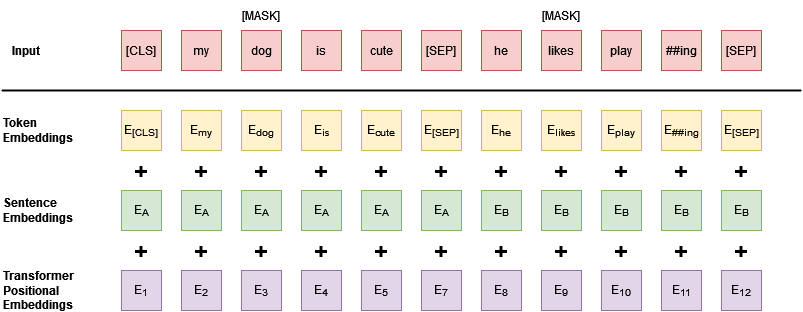
\includegraphics [height=0.7\linewidth, angle=90]{resources/NextSentence.png} \\
        \caption{\citet{Devlin2019BERTPO}}
        \label{fig:next_sentence_large}
    \end{figure}

\begin{figure}[h]
    \centering
    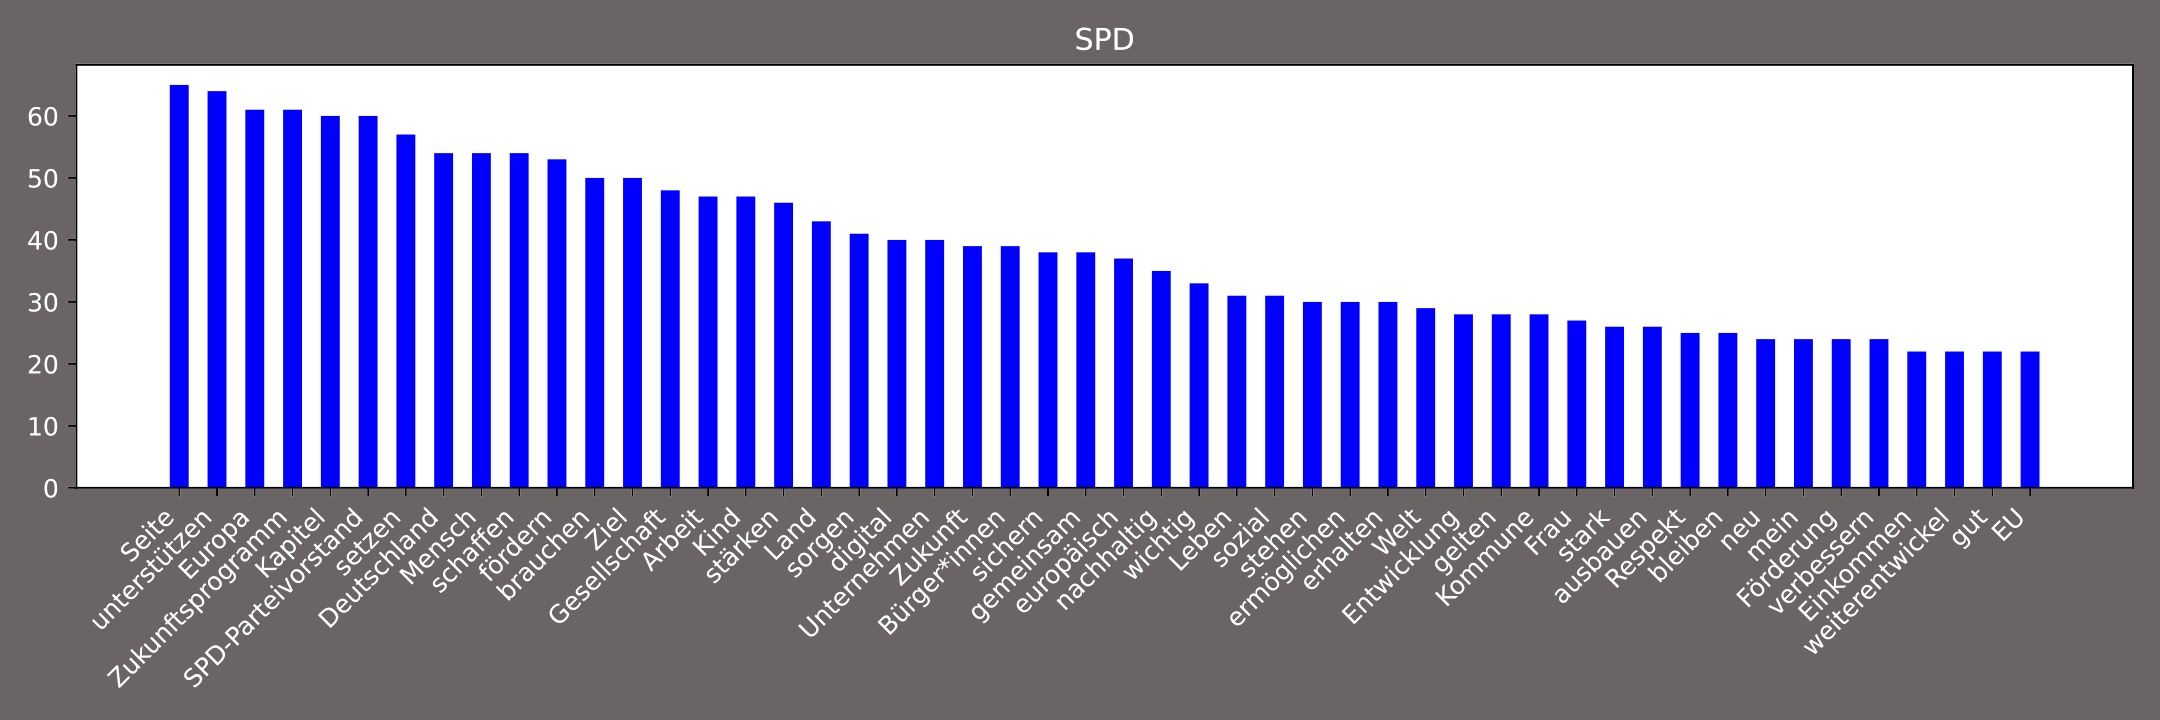
\includegraphics[height=0.7\linewidth, angle=90]{resources/graph_SPD.png}
    \caption{Word frequencies for the 50 most used words by the SPD in their 2021 federal election manifesto}
    \label{fig:spd_stats_large}
\end{figure}
\clearpage
\begin{figure}[h]
    \centering
    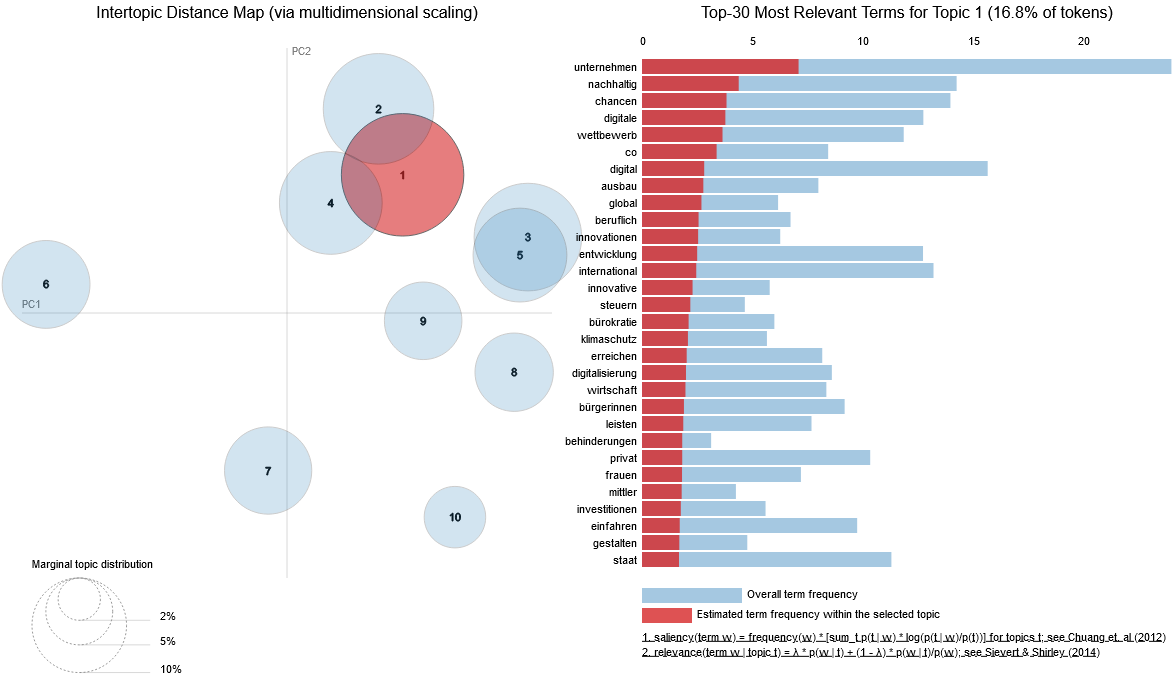
\includegraphics [height=\linewidth, angle=90]{resources/fdp_cluster.png}
    \caption{LDA visualization at the example of the FDP}
    \label{fig:lda_cluster_large}
\end{figure}

\end{document}